\documentclass{beamer}
%%%%%%%%%%%%%%%%%%%%%%%%%%%%%%%%%%%%%%%%%%%%%%%%%%%%%%%%%%%%%%%%%%%%%%%%%%%%%%
% Colours, text macros and similar stuff
%%%%%%%%%%%%%%%%%%%%%%%%%%%%%%%%%%%%%%%%%%%%%%%%%%%%%%%%%%%%%%%%%%%%%%%%%%%%%%

\usepackage{tikz}
\usetikzlibrary{calc}

%%%%%%%%%%%%%%%%%%%%%%%%%%%%%%%%%%%%%%%%%%%%%%%%%%%%%%%%%%%%%%%%%%%%%%%%%%%%%%
% Colours, text macros and similar stuff
%%%%%%%%%%%%%%%%%%%%%%%%%%%%%%%%%%%%%%%%%%%%%%%%%%%%%%%%%%%%%%%%%%%%%%%%%%%%%%

\definecolor{AltranTitle}{RGB}{139,129,120}
\definecolor{AltranSubtitle}{RGB}{115,124,130}
\definecolor{AltranGrey}{RGB}{89,89,89}

\definecolor{AnColour01}{RGB}{92,127,146} % Institutional grey
\definecolor{AnColour02}{RGB}{48,149,180} % Institutional blue

\definecolor{AnGrey01}{RGB}{213,210,202} % Warm Grey 2   - lightest
\definecolor{AnGrey02}{RGB}{199,194,186} % Warm Grey 3
\definecolor{AnGrey03}{RGB}{183,177,169} % Warm Grey 4
\definecolor{AnGrey04}{RGB}{165,157,149} % Warm Grey 6
\definecolor{AnGrey05}{RGB}{139,129,120} % Warm Grey 8   - darkest

\definecolor{AnSecondary01}{RGB}{203,0,68}   % Pinkish
\definecolor{AnSecondary02}{RGB}{190,214,0}  % Greenish
\definecolor{AnSecondary03}{RGB}{142,37,141} % Purplish
\definecolor{AnSecondary04}{RGB}{240,171,0}  % Yellowish

% Same as above with some names
\definecolor{AnSecondaryRed}{RGB}{203,0,68}      % Pinkish
\definecolor{AnSecondaryGreen}{RGB}{190,214,0}   % Greenish
\definecolor{AnSecondaryPurple}{RGB}{142,37,141} % Purplish
\definecolor{AnSecondaryYellow}{RGB}{240,171,0}  % Yellowish

% A very light grey for pxcode
\definecolor{CodeBG}{rgb}{0.95,0.95,0.95}

% Backwards compatibility
\definecolor{PraxisPurple}{RGB}{48,149,180}  % AnColour02
\definecolor{PraxisPink}{RGB}{92,127,146}    % AnColour01

\newcommand{\company}[0]{Altran}
\newcommand{\companyFormal}[0]{Altran UK Limited}
\newcommand{\companyAddress}[0]{22 St Lawrence Street, SouthGate, Bath, BA1 1AN}


\newcommand{\spark}[0]{{\sc Spark}}

\newcommand{\gps}[0]{GPS}

\newcommand{\checker}[0]{Checker}
\newcommand{\examiner}[0]{Examiner}
\newcommand{\isabelle}[0]{Isabelle/HOL}
\newcommand{\pogs}[0]{POGS}
\newcommand{\riposte}[0]{Riposte}
\newcommand{\simplifier}[0]{Simplifier}
\newcommand{\sparkclean}[0]{SPARKClean}
\newcommand{\sparkformat}[0]{SPARKFormat}
\newcommand{\sparkmake}[0]{SPARKMake}
\newcommand{\sparksimp}[0]{SPARKSimp}
\newcommand{\victor}[0]{Victor}
\newcommand{\zombiescope}[0]{ZombieScope}

\usepackage{listings}

\font\btt=cmbtt8
\lstdefinestyle{pxstyle}
   {basicstyle=\scriptsize\ttfamily,
    keywordstyle=\btt\color{AnColour02},
    commentstyle=\rmfamily\it\color{AltranGrey},
    captionpos=b,
    caption={},label={},
    numbers=none,
    escapeinside={(*}{*)}}

\lstset{defaultdialect=[LaTeX]TeX}

\lstdefinelanguage{fdl}{
  morekeywords={function,type,array,record,const,pending,var,and,or,not,for_some,for_all,
                element,update,
                may_be_replaced_by,may_be_deduced,may_be_deduced_from,are_interchangeable,if,
                goal,checktype},
  morecomment=[s]{/*}{*/}
}

%% Needs dialects for SPARK83, SPARK95 and SPARK2005
%% and some work on getting the annotation keywords to be highlighted (pun intended)
\lstdefinelanguage{SPARK}{
  language = [95]Ada,
  morekeywords = {pre,post,assert,assume,check,derives,hide,global,depends,inherit,from,own,initializes,main_program,assert,loop_variant,loop_invariant,increases,decreases,ghost,abstract_state,refined_state,refined_global,refined_depends},
  comment=[l][commentstyle]{--\ },
  texcl=true,
  showstringspaces=false
}

\lstdefinelanguage{SMTLIB}{
  language = LISP,
  morekeywords = {set-logic,
                  declare-const,declare-fun,define-const,define-fun,
                  check-sat,
                  get-value,
                  exit},
  texcl=true,
  showstringspaces=false
}


\lstdefinelanguage{indexfile}{
  morekeywords = {spec,is,in,body,specification,superindex,auxindex,components,are},
  comment=[l][commentstyle]{--\ },
  texcl=true,
  showstringspaces=false
}

\lstdefinelanguage{cmdline}{
  comment=[l][commentstyle]{--\ },
  texcl=true,
  showstringspaces=false
}

\lstnewenvironment{pxcode}[1][\@empty]{
  \lstset{language=}
  \lstset{style=pxstyle}
  \ifx#1\@empty\else
  \lstset{#1}
  \fi
}{%
}

\lstset{style=pxstyle}

\lstdefinelanguage{BNF}{
  language = [2005]Ada,
  deletecomment = [l]{--},
  morekeywords = {check,assert,pre,post},
  moredelim=[is][\emph]{//}{//},
}

% A smaller style than default, this is useful if you have a lot of
% code to typeset on a slide
\lstdefinestyle{tinystyle}
   {basicstyle=\tiny\tt,
    keywordstyle=\color{AnColour02},
    commentstyle=\rmfamily\it\color{AltranGrey},
    captionpos=b,
    caption={},label={},
    numbers=none,
    escapeinside={(*}{*)}}


\newenvironment{changemargin}[2]{%
  \begin{list}{}{%
    \setlength{\topsep}{0pt}%
    \setlength{\leftmargin}{#1}%
    \setlength{\rightmargin}{#2}%
    \setlength{\listparindent}{\parindent}%
    \setlength{\itemindent}{\parindent}%
    \setlength{\parsep}{\parskip}%
  }%
  \item[]}{\end{list}}

%%%%%%%%%%%%%%%%%%%%%%%%%%%%%%%%%%%%%%%%%%%%%%%%%%%%%%%%%%%%%%%%%%%%%%%%%%%%%%
% Altran style
%%%%%%%%%%%%%%%%%%%%%%%%%%%%%%%%%%%%%%%%%%%%%%%%%%%%%%%%%%%%%%%%%%%%%%%%%%%%%%

% We are going to position text at absolute positions on each frame.
\usepackage{textpos}

% Provide an optional \subtitle command
\gdef\thesubtitle{\ }
\def\subtitle#1{\gdef\thesubtitle{#1\\}}

% Use square shapes (in particular for bullet points)
\useinnertheme{rectangles}
\usecolortheme[named=AnColour02]{structure}    % Lighter

\setbeamercolor{block title}{use=structure,fg=white,bg=structure}
\setbeamercolor{block body}{parent=normal text,use=block title,bg=AnGrey01!40}


% The frametitle is not put in the top-left corner, but is a bit
% offset.
\setbeamertemplate{frametitle}
{
  \begin{textblock*}{\textwidth}(-0.5cm,0.5cm)
    {\rm\insertframetitle}\\
    \vskip -2mm
    {\color{AltranSubtitle}\small\insertframesubtitle}
  \end{textblock*}
  \vskip1cm
}

% No navigation symbols
\setbeamertemplate{navigation symbols}{}

% Use Altran colours throughout
\setbeamercolor*{palette quaternary}{bg=AnColour01,fg=white} % Top part

% Standard background picture
\usebackgroundtemplate{%
\begin{tikzpicture}
\node[minimum width=\paperwidth,minimum height=\paperheight-0.1pt] (page) {};
\coordinate (origin) at ($(page.south west) + (0pt, 0pt)$);
\coordinate (a) at ($(origin) + 0.9*(0cm, 1cm)$);
\coordinate (b) at ($(origin) + 0.9*(1.07cm, 0.26cm)$);
\coordinate (c) at ($(origin) + 0.9*(2.5cm, 0cm)$);
\draw[fill,AnColour02] (a) -- (b) -- (origin) -- cycle;
\draw[fill,AnGrey01] (origin) -- (b) -- (c) -- cycle;
\node[anchor=south east] at (page.south east) {
\includegraphics[width=2cm]{altran_rgb.pdf}};
\end{tikzpicture}%
}

% Page number in white
\defbeamertemplate*{footline}{AltranFooter}
{
  \hskip0.2cm{\color{white}\insertframenumber}%
  \vskip0.35cm
}
\usebeamertemplate{AltranFooter}

\setbeamertemplate{note page}
{
  \vskip0.5cm
  \begin{changemargin}{-0.5cm}{-0.5cm}
    \scriptsize\setlength\parskip{3pt}
    \insertnote
  \end{changemargin}
}


% Title page stuff.
\renewcommand{\titlepage}
{
  \begin{textblock*}{\textwidth}(0cm,-2cm)
    \flushright
    {
      \LARGE
      \color{AltranTitle}
      \rm
      \inserttitle\\
    }
    \vspace{0.1cm}
    \begin{minipage}{7.5cm}
      \flushright
      \color{AltranSubtitle}
      \thesubtitle
    \end{minipage}\\
    \vspace{0.1cm}
    {
      \scriptsize
      \insertdate
    }
  \end{textblock*}
}

\def\titleprismlabela#1{\gdef\tprismla{#1}}
\def\titleprismlabelb#1{\gdef\tprismlb{#1}}
\def\titleprismlabelc#1{\gdef\tprismlc{#1}}

\newenvironment{altrantitle}
{
  \gdef\tprismla{SPARK}
  \gdef\tprismlb{Correctness by Construction}
  \gdef\tprismlc{Formal Methods}
}
{
  {
    \usebackgroundtemplate{
\includegraphics[width=\paperwidth]{pres_title.png}}
    \begin{frame}
      \titlepage
      \begin{textblock*}{4cm}(-3.3cm,-1.5cm)
        \tiny\flushright\tprismla
      \end{textblock*}
      \begin{textblock*}{4cm}(0.6cm,3.6cm)
        \tiny\tprismlb
      \end{textblock*}
      \begin{textblock*}{4cm}(4cm,2.7cm)
        \tiny\tprismlc
      \end{textblock*}
    \end{frame}
  }
}

\renewcommand{\maketitle}{
  \begin{altrantitle}
  \end{altrantitle}
}

% The backpage is automatically added as the last slide
\newcommand{\finalslide}
{
  \usebackgroundtemplate{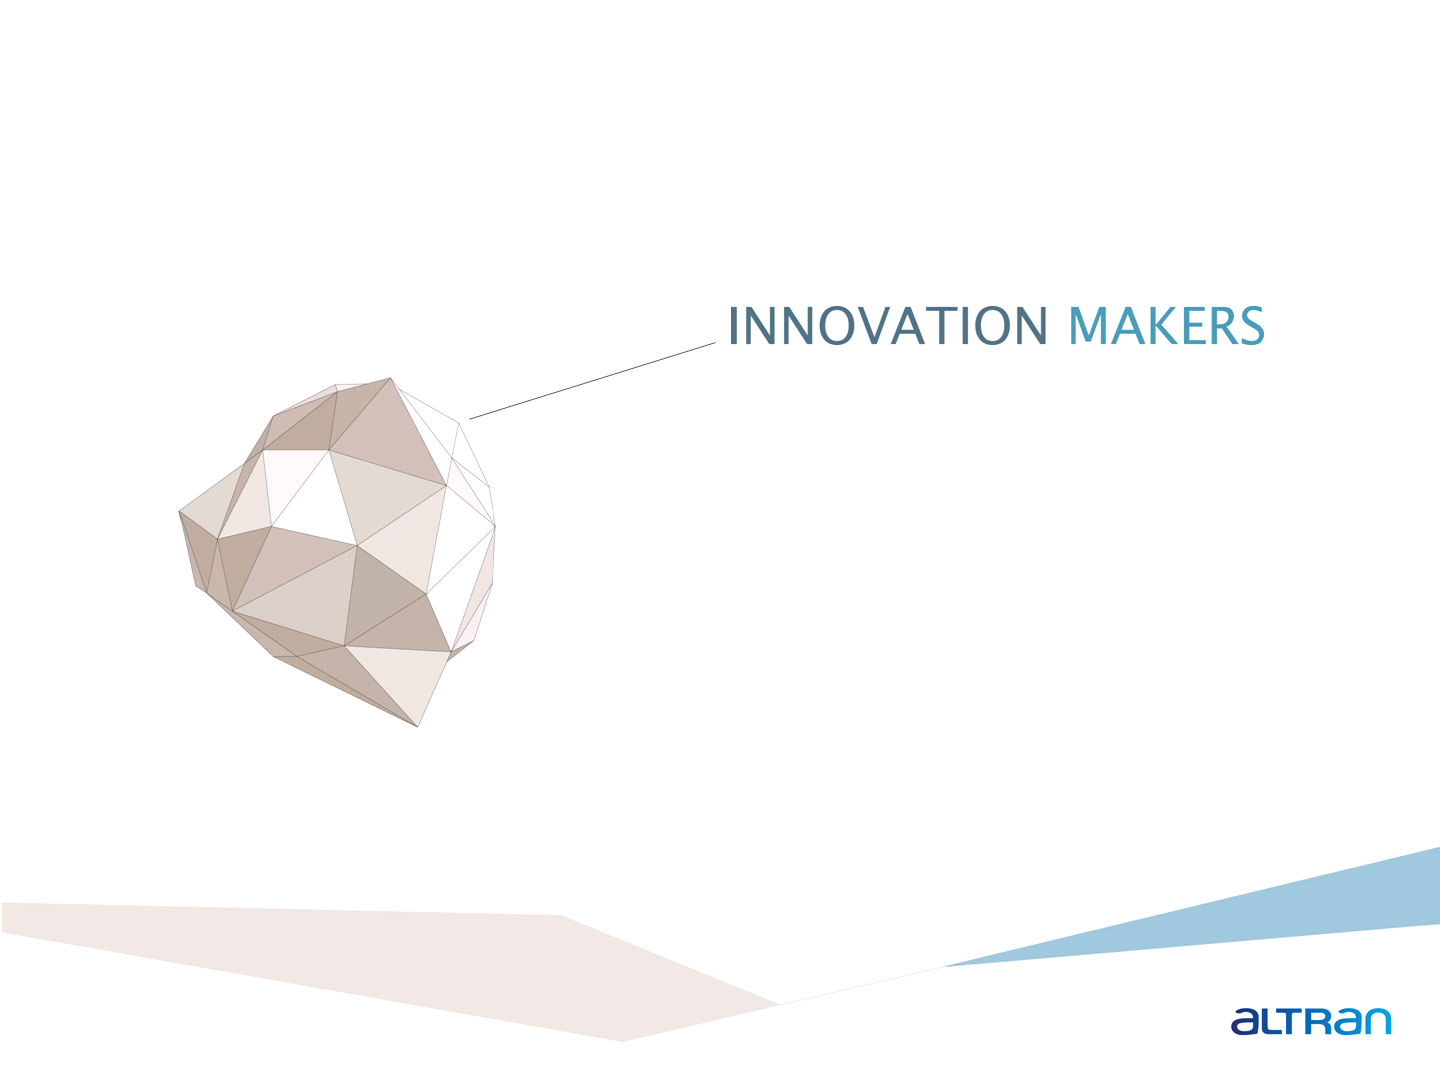
\includegraphics[width=\paperwidth]{pres_back.png}}
  \begin{frame}
  \end{frame}
}
\AtEndDocument{\finalslide}

\usepackage{listings}
\usepackage{setspace}
\usepackage{tikz}
\usetikzlibrary{calc}
\usetikzlibrary{shadows}

\lstdefinestyle{tinystyle} {basicstyle=\scriptsize\tt,
  keywordstyle=\bf, commentstyle=\rmfamily\it, escapeinside={(*}{*)}}
\lstset{style=tinystyle}

\lstdefinelanguage{SPARK}{ language = [95]Ada, morekeywords = {pre,
    post, assert, assume, check, derives, hide, global, inherit, from,
    own, initializes, main_program, input, output, in_out,
    refined_pre, refined_post, some, depends}, comment=[l][commentstyle]{--\ },
  showstringspaces=false }

\lstset{language=SPARK}

\title{Optimising Verification Effort\\with SPARK 2014}
\author{Andrew Hawthorn}
\hypersetup{colorlinks=true}
\begin{document}

\begin{altrantitle}
  \titleprismlabela{Formally Specify}
  \titleprismlabelb{Test and Prove}
  \titleprismlabelc{Reduce Cost}
\end{altrantitle}

%\begin{frame}[fragile]{Contents}
%  \tableofcontents
%\end{frame}

\makeatletter
\newenvironment{btHighlight}[1][]
{\begingroup\tikzset{bt@Highlight@par/.style={#1}}\begin{lrbox}{\@tempboxa}}
{\end{lrbox}\bt@HL@box[bt@Highlight@par]{\@tempboxa}\endgroup}

\newcommand\btHL[1][]{%
  \begin{btHighlight}[#1]\bgroup\aftergroup\bt@HL@endenv%
}
\def\bt@HL@endenv{%
  \end{btHighlight}%
  \egroup
}
\newcommand{\bt@HL@box}[2][]{%
  \tikz[remember picture]{%
    \pgfpathrectangle{\pgfpoint{1pt}{0pt}}{\pgfpoint{\wd #2}{\ht #2}}%
    \pgfusepath{use as bounding box}%
    \node[anchor=base west,%
          outer sep=0pt,%
          inner xsep=1pt,%
          inner ysep=0pt,%
          rounded corners=2pt,%
          minimum height=\ht\strutbox+1pt,%
          #1]%
          {%
            \raisebox{1pt}{\strut}\strut\usebox{#2}%
          };%
  }%
}
\makeatother

\section{Introduction}

\begin{frame}[fragile]{Key messages}
  \begin{itemize}
  \item Precision of contracts can be tailored to project need
  \item LLRs can be represented in Ada package specifications
  \item Test and proof can be easily combined

  \end{itemize}
\end{frame}

\begin{frame}[fragile]{Agenda}
  \begin{itemize}
     \item Technical planning (REVEAL, INFORMED, V-lifecylce)
     \item Verification spectrum (checks with traffic lights on left, code on right, demonstrate each level of verification with an error - start with full Ada)
     \item Example code: Presenter and audience counter (first is more precise)o
     \item ask audience to id faults? Give them a 10-second count=down timer.
  \end{itemize}
\end{frame}

\section{What?}

\begin{frame}[fragile]{Static Analysis Summary}

  \lstdefinestyle{magic}{
    basicstyle=\tiny\tt,
    keywordstyle=\color{AnColour02},
    moredelim=**[is][{\btHL[fill=AnSecondaryYellow!50,name=error]}]{`}{`},
  }

  \begin{columns}
    \begin{column}{2cm}
      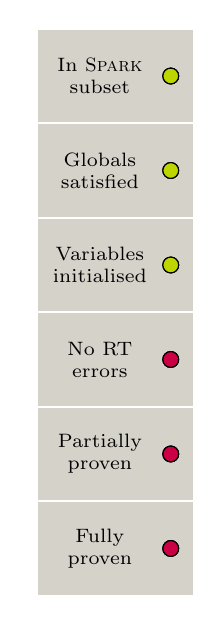
\begin{tikzpicture}[x=1cm,y=1.2cm]
        \tikzstyle{legend}=[font=\scriptsize,text badly centered,text width=1.6cm]
        \tikzstyle{unused}=[fill=white]
        \tikzstyle{error}=[fill=AnSecondaryRed]
        \tikzstyle{ok}=[fill=AnSecondaryGreen]

        \foreach \y in {1, 2, 3, 4, 5, 6} {
          \draw[fill=AnGrey01] (0, \y) -- (2, \y) -- (2, \y + 1) -- (0, \y + 1) -- (0, \y);
          \draw[white,thick]   (0, \y) -- (2, \y) -- (2, \y + 1) -- (0, \y + 1) -- (0, \y);
        }

        \node[legend] at (0.8, 6.5) {In \spark\ subset};
        \node[legend] at (0.8, 5.5) {Globals satisfied};
        \node[legend] at (0.8, 4.5) {Variables initialised};
        \node[legend] at (0.8, 3.5) {No RT errors};
        \node[legend] at (0.8, 2.5) {Partially proven};
        \node[legend] at (0.8, 1.5) {Fully\\proven};

        \draw<-1>[unused] (1.7, 6.5) circle (0.1cm);
        \draw<2>[error]   (1.7, 6.5) circle (0.1cm);
        \draw<3->[ok]     (1.7, 6.5) circle (0.1cm);

        \draw<-1>[unused]  (1.7, 5.5) circle (0.1cm);
        \draw<2>[error]    (1.7, 5.5) circle (0.1cm);
        \draw<3->[ok]      (1.7, 5.5) circle (0.1cm);

        \draw<-1>[unused] (1.7, 4.5) circle (0.1cm);
        \draw<2>[error]   (1.7, 4.5) circle (0.1cm);
        \draw<3->[ok]     (1.7, 4.5) circle (0.1cm);

        \draw<-1>[unused] (1.7, 3.5) circle (0.1cm);
        \draw<2>[error]   (1.7, 3.5) circle (0.1cm);
        \draw<3->[error]     (1.7, 3.5) circle (0.1cm);

        \draw<-1>[unused] (1.7, 2.5) circle (0.1cm);
        \draw<2>[error]   (1.7, 2.5) circle (0.1cm);
        \draw<3->[error]     (1.7, 2.5) circle (0.1cm);

        \draw<-1>[unused] (1.7, 1.5) circle (0.1cm);
        \draw<2>[error]   (1.7, 1.5) circle (0.1cm);
        \draw<3->[error]     (1.7, 1.5) circle (0.1cm);
      \end{tikzpicture}
    \end{column}

    \begin{column}{9cm}
      %\hrule

      \begin{onlyenv}<1>
      \begin{pxcode}[language=SPARK,style=magic,gobble=8]
        package Conference_Attendance
        is
           Max_Attendance : constant := 1000;
           type Count_T is range 0 .. Max_Attendance;
           Audience_Count, Presenter_Count : Count_T := 0;
           Presenter_Set : Name_Sets.Set;

           procedure Inc_Audience (N : Integer)
           with Global => (In_Out => Audience_Count),
                Pre    => (N >= 0, Audience_Count + N <= Max_Attendance),
                Post   => (Audience_Count = Audience_Count + N);

           procedure Inc_Presenter(Name : String)
           with Global => (In_Out => Presenter_Count, Presenter_List),
                Pre    => (Presenter_Count < Max_Attendance);
                Post   => (Presenters_Set.Insert(Name) and 
                           Presenter_Count = Presenters_Set.Count);
           ...


        package body Conference_Attendance
        is
           procedure Inc_Audience (N : Integer)
           is
           begin
              Audience_Count := Audience_Count - N;
           end Inc_Audience;

           ...

      \end{pxcode}
      \end{onlyenv}

      \begin{onlyenv}<2>
      \begin{pxcode}[language=SPARK,style=magic,gobble=8]
        package Conference_Numbers
        is
           A_Count, P_Count : Integer := 0;

           procedure Inc_Audience (N : Integer)
           with Global => (`In_Out => A_Count`),
                Pre    => (N >= 0),
                Post   => (A_Count = A_Count + N);
        end Counters;

        package body Counters
        is
           procedure Inc_Audience (N : Integer)
           is
           begin
              A_Count := A_Count + N;
           end Inc_Audience;
        end Counters;
      \end{pxcode}
      \end{onlyenv}

      \begin{onlyenv}<3>
      \begin{pxcode}[language=SPARK,style=magic,gobble=8]
        package Conference_Attendance
        is
           Max_Attendance : constant := 1000;
           type Count_T is range 0 .. Max_Attendance;
           Audience_Count, Presenter_Count : Count_T := 0;
           Presenter_Set : Name_Sets.Set;

           procedure Inc_Audience (N : Integer)
           with Global => (In_Out => Audience_Count),
                Pre    => (N >= 0, Audience_Count + N <= Max_Attendance),
                Post   => (Audience_Count = Audience_Count + N);

           procedure Inc_Presenter(Name : String)
           with Global => (In_Out => Presenter_Count, Presenter_List),
                Pre    => (Presenter_Count < Max_Attendance);
                Post   => (Presenters_Set.Insert(Name) and 
                           Presenter_Count = Presenters_Set.Count);
           ...


        package body Conference_Attendance
        is
           procedure Inc_Audience (N : Integer)
           is
           begin
              Audience_Count := `Audience_Count - N`;
           end Inc_Audience;

           ...
      \end{pxcode}
      \end{onlyenv}

      %\hrule
    \end{column}
  \end{columns}

\end{frame}

\end{document}

